\documentclass[12pt]{article}
\usepackage{helvet}
\usepackage{graphicx}
\usepackage{geometry}
\geometry{
    a4paper,
    top = 2cm,
    left = 2cm,
    right = 2cm,
    bottom = 3cm
}
\usepackage[utf8]{inputenc}
\usepackage[spanish,mexico]{babel} % Renombra en automático los elementos a español
\addto\captionsspanish{
  \renewcommand{\figurename}{Imagen}
  \renewcommand{\tablename}{Tabla}
}
\usepackage{float}  % Etiqueta 'H' (mayus) en figuras (imágenes)
\usepackage{array}  % Padding en tablas
\usepackage{tabularx}
\usepackage{url}    % Etiqueta url en .bib
\usepackage{booktabs}   % Manejo de caudros (tablas)
\usepackage[T1]{fontenc}    % Codificación de fuentes
\usepackage[autostyle, spanish=mexican]{csquotes}       % Paquete para comillas tipográficas
\usepackage{comment}    % Comentar bloques de líneas mediante begin-end
\usepackage{multicol}   % Para poner contenido a doble columna
\usepackage{enumitem}   % Para utilizar [noitemsep, topsep=0pt] en itemize
\usepackage{amsmath}
\usepackage{mathabx} % Para testar en math mode
\usepackage{comment}
\usepackage{longtable}
\usepackage[hidelinks]{hyperref}
\usepackage{caption}
\usepackage[
  backend=biber,
  style=apa,
  sorting=nyt
]{biblatex}
\DeclareLanguageMapping{spanish}{spanish-apa}
\renewcommand{\familydefault}{\sfdefault}
\newenvironment{localsubgroup}
  {$\left\{\tabular{l}}
  {\endtabular\right.$}


\addbibresource{bibliography/t04.bib}

\begin{comment}
Indicaciones del profesor:
Investigar sistemas de archivos (FILE SYSTEM)

- Define qué es un archivo y sus características.
- Escribe una lista de 50 diferentes tipos de archivos de acuerdo a su extensión y con cuál programa se crea y modifica. Ej. PDF es utilizada con Acrobat Reader.
- Define qué es un FILE SYSTEM y realiza una tabla 10 distintos FS y sus características principales.
- Qué es FS utiliza GNU/Linux Mint 21.2 "Victoria", Ubunut 23.04, MacOS Catalina y Microsoft Windows 10 en la actualidad.

Un máximo de 25 hojas.

Rango de páginas exigido: mínimo 18 páginas, máximo 25 páginas (límite estricto por indicación docente). Objetivo: 22 a 24 páginas.

Índice aprobado y presupuesto de páginas:
1. Definición y características de los archivos (~3.5 págs.)
2. Taxonomía y catálogo de formatos de archivo (~5.0 págs.)
3. Arquitectura y componentes de los sistemas de archivos (~4.0 págs.)
4. Análisis comparativo de sistemas de archivos (~3.5 págs.)
5. Sistemas de archivos en sistemas operativos contemporáneos (~3.5 págs.)
6. Conclusiones personales (~2.0 págs. monolíticas)
Referencias (~1.0 pág.)
Total estimado: 22.5 - 24.0 páginas (dentro del rango reglamentario 18 a 25 páginas).
\end{comment}

\begin{document}
\pagenumbering{roman}

\begin{titlepage}
  \thispagestyle{empty}
  \newgeometry{left = 1cm, right = 1cm, top = 1cm, bottom = 2cm}

  \noindent
  \begin{minipage}[c]{3.5cm}
    
\includegraphics[width=3.5cm]{media/titlepage/Escudo-UNAM.pdf}
  \end{minipage}\hfill
  \begin{minipage}[c][3.5cm][c]{\dimexpr\textwidth-7cm\relax}
    \centering
    {\large\textbf{Universidad Nacional Autónoma de México}\\[0.6em] 
    \Large\textbf{Facultad de Ingeniería}\\[0.6em]
    \large Sistemas Operativos}
  \end{minipage}\hfill
  \begin{minipage}[c]{3.5cm}
    \raggedleft
    
\includegraphics[width=3.5cm]{media/titlepage/FI.png}
  \end{minipage}
\centering\huge
  \vfill
    Grupo 1 \\
    Ing. Angel Isidro Mercado
  \vfill
    \textbf{Tarea 4. Sistemas de Archivos}
  \vfill\large
    320304435 - Cabrera Rojas Oscar
  \vfill

  \noindent\footnotesize \hfill Ciudad Universitaria, CDMX a 02 de octubre del 2026
\end{titlepage}
\restoregeometry

\tableofcontents

\newpage
\pagenumbering{arabic}
\setcounter{page}{1}

\section{Definición y características de los archivos}
\label{sec:definicionCaracteristicasArchivos}

\subsection{Concepto y naturaleza lógica del archivo}
\label{subsec:conceptoNaturalezaArchivo}

El subsistema de gestión de almacenamiento es uno de los componentes más visibles y fundamentales dentro de la arquitectura de cualquier sistema operativo moderno. Desde la perspectiva del usuario y de las aplicaciones en ejecución, la memoria de acceso aleatorio (RAM, \textit{Random Access Memory}) resulta un medio volátil, de capacidad acotada y dependiente del suministro ininterrumpido de energía eléctrica, lo que impide la conservación indefinida del estado de los programas y sus datos. Para resolver esta limitación, el sistema operativo implementa una abstracción uniforme sobre los dispositivos físicos de almacenamiento secundario no volátil (discos magnéticos, unidades de estado sólido basadas en memorias flash NAND, medios ópticos o arreglos en red), ocultando la topología de sectores, bloques físicos, pistas y comandos de bajo nivel del controlador de hardware \parencite[\S 10.1, p.\ 333]{silberschatz2006fundamentos}.

Formalmente, un archivo es una colección con nombre de información relacionada, representada como una secuencia contigua en el espacio de direcciones lógicas y almacenada de forma persistente en memoria secundaria \parencite[\S 8.2.1, p.\ 421]{carretero2001sistemas}. El archivo constituye la unidad lógica mínima de asignación y persistencia que el sistema operativo expone al usuario; ninguna aplicación puede almacenar datos en un medio persistente sin asociarlos a la entidad de un archivo reconocido por el sistema \parencite[\S 10.1, p.\ 333]{silberschatz2006fundamentos}. Esta entidad posee propiedades indispensables:
\begin{itemize}[noitemsep, topsep=2pt]
    \item \textbf{Persistencia temporal prolongada:} la información subsiste a la terminación del proceso que la generó, al cierre de la sesión del usuario e incluso a reinicios abruptos o fallos en el suministro eléctrico del equipo anfitrión \parencite[\S 12.1, p.\ 551]{stallings2018operating}.
    \item \textbf{Identificación simbólica e independencia:} el archivo posee un nombre textual independiente del proceso creador, lo que permite su localización, referenciación y transferencia a través de diferentes entornos informáticos \parencite[\S 10.1.1, p.\ 334]{silberschatz2006fundamentos}.
    \item \textbf{Control de concurrencia y coutilización:} dispone de mecanismos de sincronización, cerrojos y derechos de acceso que permiten a múltiples procesos compartir datos de manera coordinada y segura \parencite[\S 13.3, p.\ 587]{deitel2004operating}.
\end{itemize}

En el diseño de sistemas operativos coexisten dos paradigmas arquitectónicos para modelar el contenido interno de un archivo: el enfoque basado en registros estructurados y el enfoque orientado a flujo continuo de bytes. En sistemas operativos heredados de computadoras centrales (\textit{mainframes}) y entornos de procesamiento transaccional como IBM z/OS o DEC VMS, los archivos se conciben bajo una jerarquía estricta compuesta por campos elementales que forman registros lógicos de longitud fija o variable \parencite[\S 13.2, pp.\ 586--587]{deitel2004operating}. En dicho modelo, el propio núcleo del sistema operativo comprende la delimitación de cada registro, proveyendo primitivas de lectura orientadas a unidades de registro completas. No obstante, esta aproximación sobrecarga el núcleo con una proliferación excesiva de rutinas de soporte para cada tipo de dato, restringiendo la interoperabilidad cuando surgen aplicaciones con formatos no previstos por los diseñadores del sistema operativo \parencite[\S 10.1, p.\ 341]{silberschatz2006fundamentos}.

Por el contrario, el modelo introducido por UNIX y consolidado en los estándares de la interfaz de sistema operativo portátil (POSIX, \textit{Portable Operating System Interface}), adoptado igualmente por Windows y los núcleos modernos de Linux y BSD, concibe el archivo como una secuencia lineal no estructurada de bytes de 8 bits (\textit{stream of bytes}) \parencite[\S 8.2.1, pp.\ 421--422]{carretero2001sistemas}. Para el núcleo, el contenido de un archivo es semánticamente agnóstico y carece de estructura predeterminada; cada byte es accesible mediante su desplazamiento numérico relativo al inicio. La responsabilidad de interpretar, segmentar y validar el flujo binario recae exclusivamente en las bibliotecas de tiempo de ejecución y en la lógica de las aplicaciones de usuario \parencite[\S 10.1, p.\ 341]{silberschatz2006fundamentos}. Esta ortogonalidad provee la máxima flexibilidad y simplifica el diseño del núcleo, permitiendo tratar de forma análoga archivos ordinarios, tuberías de comunicación y descriptores de dispositivos físicos bajo la premisa universal de que \enquote{en UNIX, todo es un archivo}.

A nivel físico, el hardware de almacenamiento opera invariablemente transfiriendo bloques de datos de tamaño homogéneo (comúnmente sectores lógicos de 512 bytes o bloques de 4096 bytes en formatos avanzados). El subsistema de archivos se encarga de empaquetar de forma transparente los bytes del flujo lógico dentro de los bloques físicos asignados. Cuando la longitud total de los datos no coincide con un múltiplo exacto del tamaño de bloque, la porción residual del último bloque queda sin utilizarse, fenómeno denominado fragmentación interna \parencite[\S 10.1.5, p.\ 342]{silberschatz2006fundamentos}.

\subsection{Atributos y metadatos del archivo}
\label{subsec:atributosMetadatosArchivo}

Un archivo no se limita a su cuerpo de datos; el sistema operativo asocia y preserva de manera inseparable un conjunto de metadatos o atributos de control que describen su estado, permisos, procedencia y ubicación física en el medio \parencite[\S 12.1, p.\ 552]{stallings2018operating}. Estos metadatos permiten a los subsistemas de seguridad, planificación y memoria administrar el archivo con eficiencia e integridad. Los atributos universales presentes en los sistemas contemporáneos son:

\begin{enumerate}[noitemsep, topsep=2pt]
    \item \textbf{Nombre simbólico:} Cadena de caracteres alfanuméricos destinada a la interacción con el usuario y la jerarquía de directorios. En sistemas con distinción de mayúsculas y minúsculas (\textit{case-sensitive}) como Linux, \texttt{informe.txt} y \texttt{Informe.txt} constituyen archivos distintos, mientras que en sistemas insensibles a las mayúsculas como NTFS en Windows son equivalentes.
    \item \textbf{Identificador unívoco:} Valor numérico binario único que identifica inequívocamente al archivo dentro de la estructura física del sistema de archivos \parencite[\S 10.1.1, p.\ 334]{silberschatz2006fundamentos}. En sistemas POSIX corresponde al número de nodo de índice (\textit{inode} o inodo), mientras que en NTFS de Windows se materializa en el índice del registro de la tabla maestra de archivos (MFT, \textit{Master File Table}) \parencite[\S 8.2.1, p.\ 422]{carretero2001sistemas}. Las estructuras internas del núcleo operan siempre mediante este identificador numérico, independientemente del nombre simbólico o las rutas de acceso.
    \item \textbf{Tipo de archivo y formato:} Especifica la naturaleza intrínseca del archivo. En entornos de escritorio se apoya en extensiones de archivo o identificadores de tipo MIME (\textit{Multipurpose Internet Mail Extensions}). No obstante, en el nivel del núcleo se recurre al denominado número mágico (\textit{magic number}), una secuencia fija de bytes grabada en los primeros sectores de la cabecera del archivo que valida inequívocamente su formato (por ejemplo, los bytes \texttt{0x7F 0x45 0x4C 0x46} para binarios ELF en Linux o \texttt{0x25 0x50 0x44 0x46} para documentos PDF) \parencite[\S 8.2.1, p.\ 422]{carretero2001sistemas}.
    \item \textbf{Ubicación y mapa de asignación:} Punteros y estructuras de direccionamiento que relacionan el espacio lógico del archivo con los identificadores de bloques lógicos (LBA, \textit{Logical Block Addressing}) o agrupaciones de sectores (\textit{clusters}) en el dispositivo físico de almacenamiento \parencite[\S 8.2.1, p.\ 422]{carretero2001sistemas}.
    \item \textbf{Tamaño y consumo de almacenamiento:} Describe tanto la longitud lógica actual del archivo en bytes como la cantidad real de bloques físicos reservados en disco. En archivos dispersos (\textit{sparse files}), el tamaño lógico puede ser de varios terabytes mientras que el espacio físico consumido se reduce a los pocos bloques que contienen datos distintos de cero.
    \item \textbf{Control de acceso y protección:} Información de privilegios que dictamina qué entidades pueden ejecutar operaciones de lectura, escritura o ejecución. En entornos POSIX se implementa mediante la máscara clásica de nueve bits (lectura, escritura y ejecución para usuario propietario, grupo y otros), complementada por listas de control de acceso (ACL, \textit{Access Control Lists}) que permiten asignar derechos granulares a usuarios o grupos individuales \parencite[\S 12.1, pp.\ 552--553]{stallings2018operating}.
    \item \textbf{Marcas temporales (\textit{timestamps}):} Registros cronológicos de auditoría que documentan eventos críticos del ciclo de vida del archivo. En sistemas tipo UNIX y Linux se distinguen tres marcas elementales:
    \begin{itemize}[noitemsep, topsep=1pt]
        \item \texttt{atime} (\textit{access time}): marca temporal del último acceso de lectura al contenido del archivo.
        \item \texttt{mtime} (\textit{modification time}): marca temporal de la última escritura o modificación del contenido de datos.
        \item \texttt{ctime} (\textit{change time}): marca temporal del último cambio en los metadatos o atributos del inodo (permisos, propietario, enlaces duros).
        \item En sistemas modernos y en NTFS se incorpora además \texttt{crtime} / \texttt{btime} (\textit{creation/birth time}), registrando el instante exacto en que fue creado el archivo \parencite[\S 8.2.1, p.\ 423]{carretero2001sistemas}.
    \end{itemize}
\end{enumerate}

La Tabla~\ref{tab:atributosMetadatosArchivo} sintetiza los atributos analizados, contrastando su nomenclatura conceptual con su implementación real en sistemas tipo UNIX y en entornos Windows.

\begin{table}[H]
\centering
\footnotesize
\renewcommand{\arraystretch}{1.1}
\renewcommand{\tabularxcolumn}[1]{m{#1}}
\setlength{\emergencystretch}{1.5em}
\caption{Atributos y metadatos fundamentales de los archivos en sistemas operativos contemporáneos.}
\label{tab:atributosMetadatosArchivo}
\begin{tabularx}{\textwidth}{>{\centering\arraybackslash}m{2.9cm} X X}
\toprule
\textbf{Atributo} & \textbf{Implementación en UNIX / Linux (Inodo / POSIX)} & \textbf{Implementación en Windows (MFT / NTFS)} \\
\midrule
\textbf{Identificador} & Número de inodo entero (\texttt{ino\_t}), único por partición lógica montada en el árbol. & Identificador de referencia de 64 bits compuesto por el índice en la MFT y un número de secuencia. \\
\addlinespace
\textbf{Tipo} & Campo \texttt{st\_mode} codificado en bits (archivo regular, directorio, enlace simbólico, socket, tubería, dispositivo). & Atributos de registro en MFT y asociación mediante la extensión del nombre en el Registro de Windows. \\
\addlinespace
\textbf{Seguridad} & Identificador de usuario (\texttt{uid}), de grupo (\texttt{gid}), bits \texttt{rwxrwxrwx}, SUID/SGID y atributos POSIX ACL. & Descriptor de seguridad (\textit{Security Descriptor}) que integra el SID del dueño y una lista ACL discrecional (DACL). \\
\addlinespace
\textbf{Mapa de bloques} & Árbol de punteros directos, indirectos simples, dobles y triples (o árbol de extensiones \textit{extents} en ext4). & Lista de fragmentos de ejecución (\textit{runlists}) que especifican pares de desplazamiento virtual (VCN) y lógico (LCN). \\
\addlinespace
\textbf{Temporización} & Estructuras \texttt{timespec} para marcas \texttt{atime}, \texttt{mtime} y \texttt{ctime} con resolución de nanosegundos. & Estructuras \texttt{FILETIME} de 64 bits con precisión de 100 nanosegundos para creación, modificación, acceso y cambio. \\
\bottomrule
\end{tabularx}
\end{table}

\subsection{Estructuras del núcleo y gestión de archivos abiertos}
\label{subsec:estructurasNucleoArchivosAbiertos}

Para evitar lecturas repetitivas y costosas a las estructuras de almacenamiento secundario cada vez que un proceso requiere transferir datos, el sistema operativo implementa en memoria principal una jerarquía de estructuras de control que optimizan la gestión de los archivos abiertos \parencite[\S 11.2, p.\ 372]{silberschatz2006fundamentos}.

En disco, toda la información de control y mapa de un archivo se encuentra condensada en el Bloque de Control de Archivo (FCB, \textit{File Control Block}) \parencite[\S 11.2, p.\ 373]{silberschatz2006fundamentos}. Al emitirse una solicitud de apertura mediante la llamada al sistema \texttt{open()}, el subsistema de archivos explora la estructura de directorios, valida los permisos de acceso y traslada una copia del FCB a las estructuras dinámicas del núcleo en memoria RAM. Esta coordinación se articula a través de tres niveles de abstracción:

\begin{enumerate}[noitemsep, topsep=2pt]
    \item \textbf{Tabla de descriptores de archivo por proceso:} Cada entrada en la tabla de procesos del núcleo (el Bloque de Control del Proceso o PCB) mantiene un arreglo de descriptores de archivo abiertos. El índice de este arreglo es el descriptor de archivo (\textit{file descriptor} en POSIX, un número entero no negativo; o \textit{file handle} en Windows). Esta tabla local almacena el modo de acceso asignado al descriptor y un puntero a una entrada específica dentro de la tabla global de archivos abiertos del sistema \parencite[\S 11.2, p.\ 373]{silberschatz2006fundamentos}.
    \item \textbf{Tabla global de archivos abiertos del sistema (\textit{system-wide open-file table}):} Alberga una entrada por cada archivo en uso en el sistema. Contiene el puntero de desplazamiento actual (\textit{file offset}) compartido entre los descriptores vinculados a dicha entrada (por ejemplo, tras una llamada \texttt{fork()}), el modo de acceso efectivo (\texttt{O\_RDONLY}, \texttt{O\_WRONLY}, \texttt{O\_RDWR}), el contador de referencias de aperturas activas (\textit{open count}) y un puntero hacia la estructura de nodo virtual (\textit{vnode}) o inodo en memoria activa \parencite[\S 10.1.2, p.\ 336]{silberschatz2006fundamentos}.
    \item \textbf{Tabla de inodos en memoria activa (\textit{vnode / inode table}):} Mantiene la copia sincronizada del FCB o inodo físico del disco, complementada con información puramente dinámica del núcleo: cerrojos de exclusión mutua, semáforos de sincronización, lista de páginas sucias en la memoria caché del sistema (\textit{page cache}) y contador global de enlaces duros \parencite[\S 8.6.2, p.\ 473]{carretero2001sistemas}.
\end{enumerate}

La Img.~\ref{fig:estructurasArchivosAbiertos} ilustra el flujo de punteros y estructuras de datos involucradas en la apertura y lectura coordinada de un archivo por parte de procesos independientes y procesos emparentados en el sistema operativo.

\begin{figure}[H]
    \centering
    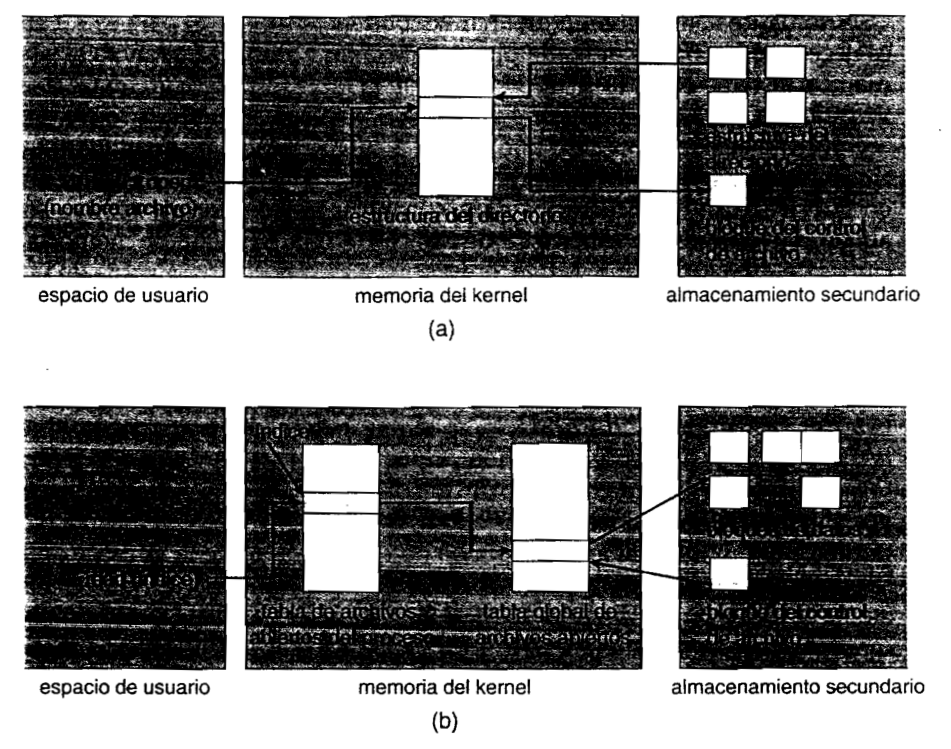
\includegraphics[width=\columnwidth]{media/t04/estructurasArchivosAbiertos.png}
    \caption{Estructuras de control en memoria del sistema operativo para la gestión coordinada de archivos abiertos \parencite[\S 11.2, p.\ 373]{silberschatz2006fundamentos}.}
    \label{fig:estructurasArchivosAbiertos}
\end{figure}

Cuando un proceso invoca la primitiva \texttt{close()}, el núcleo elimina la entrada correspondiente en la tabla del proceso y decrementa en una unidad el contador de aperturas en la tabla global. Si dos procesos independientes abrieron el mismo archivo por separado, cada uno posee su propio puntero de desplazamiento en la tabla global, evitando que la lectura efectuada por un proceso altere la posición de lectura del otro. Únicamente cuando el contador de aperturas del archivo desciende a cero, el núcleo descarga las páginas modificadas a disco (\textit{flush}), libera la entrada global y retira el inodo de la memoria activa si no existen otras referencias en caché \parencite[\S 10.1.2, pp.\ 336--337]{silberschatz2006fundamentos}.

\subsection{Operaciones del núcleo sobre archivos}
\label{subsec:operacionesNucleoArchivos}

Un archivo constituye formalmente un tipo abstracto de datos, caracterizado tanto por su estado y atributos como por el conjunto de operaciones primitivas que el sistema operativo pone a disposición de las aplicaciones mediante llamadas al sistema (\textit{system calls}) \parencite[\S 10.1.2, p.\ 335]{silberschatz2006fundamentos}. Las operaciones medulares implementadas en los núcleos contemporáneos son:

\begin{itemize}[noitemsep, topsep=2pt]
    \item \textbf{Creación (\textit{create}):} Localiza espacio libre en la estructura del sistema de archivos para alojar el nuevo FCB o inodo, inicializa sus atributos (propietario, permisos, marcas de tiempo en cero) y registra una nueva entrada en el directorio padre que vincula el nombre simbólico con el identificador numérico asignado \parencite[\S 10.1.2, p.\ 335]{silberschatz2006fundamentos}.
    \item \textbf{Apertura (\textit{open}):} Verifica los derechos de acceso del proceso solicitante contra la ACL o los permisos del inodo, carga el FCB a memoria activa si no se hallaba previamente en uso, inicializa una entrada en la tabla global del sistema y asigna un descriptor no negativo en la tabla local del proceso, retornando dicho descriptor al espacio de usuario \parencite[\S 11.2, p.\ 373]{silberschatz2006fundamentos}.
    \item \textbf{Lectura (\textit{read}):} A partir del descriptor proporcionado, consulta el puntero de desplazamiento actual, transfiere el número de bytes solicitado desde la caché de páginas del núcleo hacia el búfer de memoria del espacio de usuario y avanza el puntero de desplazamiento en una cantidad de bytes equivalente a los leídos \parencite[\S 10.1.2, p.\ 335]{silberschatz2006fundamentos}.
    \item \textbf{Escritura (\textit{write}):} Transfiere bytes desde el búfer de la aplicación hacia las páginas de caché del núcleo, asignando nuevos bloques físicos en disco si la operación supera el tamaño actual del archivo, y avanza el puntero de desplazamiento. En sistemas con escritura pospuesta (\textit{write-behind}), los datos se persisten en disco de forma asíncrona mediante demonios del núcleo (como \texttt{pdflush} o \texttt{kworker} en Linux), salvo que se invoque explícitamente una llamada de sincronización obligatoria como \texttt{fsync()} o \texttt{fdatasync()} \parencite[\S 8.4.2, p.\ 441]{carretero2001sistemas}.
    \item \textbf{Reposicionamiento (\textit{seek}):} Modifica la posición actual del puntero de desplazamiento relativo al inicio (\texttt{SEEK\_SET}), a la posición actual (\texttt{SEEK\_CUR}) o al final del archivo (\texttt{SEEK\_END}), sin llevar a cabo ninguna transferencia física de entrada/salida sobre el dispositivo \parencite[\S 10.1.2, pp.\ 335--336]{silberschatz2006fundamentos}.
    \item \textbf{Truncado (\textit{truncate}):} Reduce la longitud lógica de un archivo a un número determinado de bytes (frecuentemente cero) y devuelve al mapa de bloques libres el espacio sobrante en disco, preservando inalterados todos los metadatos, propietario y atributos de seguridad del archivo \parencite[\S 10.1.2, p.\ 335]{silberschatz2006fundamentos}.
    \item \textbf{Cierre y desvinculación (\textit{close} y \textit{unlink}):} \texttt{close()} disocia el descriptor del proceso liberando la entrada local y decrementando el contador global. Por su parte, \texttt{unlink()} o \texttt{DeleteFile()} suprime el enlace en el directorio; si el archivo no posee otros enlaces duros y su contador de aperturas es cero, el núcleo procede a liberar definitivamente todos los bloques de datos y el FCB/inodo en el medio persistente \parencite[\S 8.4.2, p.\ 442]{carretero2001sistemas}.
\end{itemize}

La Tabla~\ref{tab:llamadasSistemaArchivos} compara directamente las llamadas al sistema estandarizadas en la norma POSIX de IEEE/The Open Group frente a las interfaces de programación nativas de Win32 provistas por el subsistema del núcleo de Windows NT.

\begin{table}[H]
\centering
\footnotesize
\renewcommand{\arraystretch}{1.1}
\renewcommand{\tabularxcolumn}[1]{m{#1}}
\setlength{\emergencystretch}{1.5em}
\caption{Comparativa de interfaces de llamadas al sistema para operaciones sobre archivos: POSIX frente a Win32.}
\label{tab:llamadasSistemaArchivos}
\begin{tabularx}{\textwidth}{>{\centering\arraybackslash}m{3.6cm} X X}
\toprule
\textbf{Operación} & \textbf{Llamada al sistema POSIX (C / Linux / BSD)} & \textbf{Función de la API Win32 (Windows NT)} \\
\midrule
\textbf{Apertura y creación} & \texttt{open(path, flags, mode)} & \texttt{CreateFile(name, access, share, sec, disp, flags, temp)} \\
\addlinespace
\textbf{Lectura} & \texttt{read(fd, buf, count)} & \texttt{ReadFile(file, buf, count, bytesRead, overlapped)} \\
\addlinespace
\textbf{Escritura} & \texttt{write(fd, buf, count)} & \texttt{WriteFile(file, buf, count, bytesWritten, overlapped)} \\
\addlinespace
\textbf{Reposicionamiento} & \texttt{lseek(fd, offset, whence)} & \texttt{SetFilePointer(file, distLow, distHigh, method)} \\
\addlinespace
\textbf{Truncado} & \texttt{truncate(path, len)} o \texttt{ftruncate(fd, len)} & \texttt{SetEndOfFile(file)} tras posicionar el puntero del archivo. \\
\addlinespace
\textbf{Cierre de descriptor} & \texttt{close(fd)} & \texttt{CloseHandle(handle)} \\
\addlinespace
\textbf{Eliminación} & \texttt{unlink(path)} & \texttt{DeleteFile(name)} \\
\bottomrule
\end{tabularx}
\end{table}

\subsection{Organización interna y métodos de acceso}
\label{subsec:organizacionInternaMetodosAcceso}

La manera en que un archivo es leído y procesado por el software determina el método de acceso soportado por el sistema de archivos. Dependiendo de los requerimientos de latencia, concurrencia y ordenamiento de la aplicación, se distinguen tres métodos principales \parencite[\S 10.2, pp.\ 337--340]{silberschatz2006fundamentos}:

\begin{enumerate}[noitemsep, topsep=2pt]
    \item \textbf{Acceso secuencial:} Es el método más simple y extendido. La información contenida en el archivo se procesa en estricto orden lineal, byte por byte o registro por registro, desde el principio hasta el final \parencite[\S 12.2, p.\ 556]{stallings2018operating}. Las operaciones de lectura consumen automáticamente el siguiente segmento de datos (\texttt{read\_next}) y avanzan el puntero de archivo de manera implícita. Las operaciones de escritura añaden información de forma continua al final del archivo (\texttt{append}). Este esquema emula fielmente el comportamiento de dispositivos electromecánicos lineales como las cintas magnéticas y resulta óptimo para compiladores, analizadores de texto, volcado de registros de eventos (\textit{logs}) y reproductores continuos de audio y vídeo \parencite[\S 10.2.1, p.\ 337]{silberschatz2006fundamentos}.
    \item \textbf{Acceso directo o aleatorio (\textit{direct / random access}):} En este modelo, el archivo se concibe como una secuencia indexada de bloques de datos de tamaño homogéneo. Los programas pueden leer o escribir en cualquier bloque en un orden arbitrario, especificando el número de bloque relativo al inicio del archivo (\texttt{read\_block(n)}), o desplazando libremente el puntero mediante llamadas como \texttt{lseek()} \parencite[\S 10.2.2, p.\ 338]{silberschatz2006fundamentos}. El acceso directo es imprescindible para sistemas de gestión de bases de datos relacionales (DBMS, \textit{Database Management Systems}), almacenes clave-valor y motores de virtualización de discos rígidos, donde la aplicación requiere modificar registros dispersos sin leer exhaustivamente los datos precedentes. Asimismo, sustenta la técnica de proyección de archivos en memoria (\textit{memory-mapped files} mediante la llamada \texttt{mmap()}), permitiendo mapear páginas de un archivo directamente en el espacio de direcciones virtuales del proceso para manipular su contenido como si fuera un arreglo nativo en memoria RAM \parencite[\S 8.2.4, pp.\ 427--428]{carretero2001sistemas}.
    \item \textbf{Acceso indexado:} Diseñado para archivos de gran escala donde se requiere alta velocidad de localización basada en una clave de búsqueda (\textit{key}) \parencite[\S 12.2, pp.\ 558--560]{stallings2018operating}. El sistema mantiene un archivo de índice separado compuesto por punteros dirigidos hacia los bloques de datos del archivo principal. Para localizar un registro específico, el subsistema realiza una búsqueda binaria o recorre un árbol balanceado (árbol B o B+) sobre el índice, determinando la dirección física exacta del bloque de destino en una fracción mínima de tiempo en comparación con un barrido secuencial completo \parencite[\S 8, pp.\ 249--252]{mchoes2011sistemas}. En sistemas que atienden volúmenes masivos de información, se construyen índices multinivel donde un índice primario direcciona a subíndices secundarios antes de alcanzar los bloques finales de datos \parencite[\S 10.2.3, p.\ 339]{silberschatz2006fundamentos}.
\end{enumerate}

\section{Taxonomía y catálogo de formatos de archivo}
\label{sec:taxonomiaCatalogoFormatos}

\subsection{Mecanismos de identificación: extensiones, tipos MIME y números mágicos}
\label{subsec:mecanismosIdentificacionFormatos}

La capacidad del sistema operativo para determinar la naturaleza y estructura interna de un archivo resulta decisiva para garantizar la correcta ejecución de los programas, evitar la corrupción de datos y prevenir vulnerabilidades de seguridad derivadas de la interpretación errónea de flujos binarios \parencite[\S 10.1.3, p.\ 339]{silberschatz2006fundamentos}. A lo largo de la evolución de las arquitecturas de software, se han consolidado tres mecanismos fundamentales para la identificación y enlace de formatos:

\begin{enumerate}[noitemsep, topsep=2pt]
    \item \textbf{Extensiones de nombre de archivo:} Introducidas de forma rígida en sistemas de disco como CP/M y MS-DOS bajo el formato de 8 caracteres de nombre y 3 de sufijo (convención 8.3), las extensiones constituyen sufijos alfanuméricos anexados tras el último carácter de punto en el nombre simbólico del archivo \parencite[\S 10.1.3, p.\ 340]{silberschatz2006fundamentos}. En sistemas Windows, el subsistema gráfico y el Registro central (\texttt{HKEY\_CLASSES\_ROOT}) asocian de manera determinista cada extensión con un controlador ejecutable específico (p. ej., asociando \texttt{.pdf} con Adobe Acrobat Reader). No obstante, esta aproximación presenta debilidades estructurales: la extensión es meramente nominal y puede ser alterada arbitrariamente por el usuario o por software malicioso (p. ej., técnicas de ofuscación mediante doble extensión como \texttt{documento.pdf.exe}), induciendo al usuario a ejecutar código arbitrario creyendo abrir un documento pasivo.
    \item \textbf{Números mágicos y firmas binarias (\textit{magic numbers}):} Como contraparte a la fragilidad de las extensiones, el estándar POSIX y los sistemas basados en UNIX implementan el análisis directo de los primeros bytes de la cabecera física del archivo \parencite[\S 8.2.1, p.\ 422]{carretero2001sistemas}. Un número mágico es una secuencia estandarizada e invariable de bytes situada en un desplazamiento fijo (\textit{offset}) dentro del archivo que identifica de forma irrefutable su especificación técnica, independientemente del nombre asignado. El comando estándar \texttt{file} y la biblioteca del sistema \texttt{libmagic} operan consultando bases de datos de patrones estructurados (\texttt{/etc/magic}), permitiendo reconocer ejecutables binarios ELF (\texttt{0x7F 0x45 0x4C 0x46}), imágenes PNG (\texttt{0x89 0x50 0x4E 0x47 0x0D 0x0A 0x1A 0x0A}) o contenedores ZIP (\texttt{0x50 0x4B 0x03 0x04}) incluso si el archivo carece de extensión o ha sido renombrado maliciosamente.
    \item \textbf{Tipos de medios de Internet (MIME / IANA):} Estandarizados originalmente en la RFC 2046 por el IETF para el intercambio estructurado de correo electrónico multimedia \parencite{freed1996multipurpose}, los tipos MIME representan una taxonomía universal en dos niveles (\texttt{tipo/subtipo}, como \texttt{text/plain}, \texttt{application/pdf} o \texttt{image/png}). En entornos de escritorio contemporáneos como GNOME y KDE bajo especificaciones de Freedesktop.org, el subsistema Shared MIME-Info combina heurísticas de extensión con inspección de números mágicos para despachar aplicaciones de forma unificada mediante descriptores \texttt{.desktop} y archivos de configuración \texttt{mimeapps.list}.
\end{enumerate}

\subsection{Catálogo técnico clasificado de cincuenta formatos de archivo}
\label{subsec:catalogoCincuentaFormatos}

A continuación se presenta un catálogo técnico exhaustivo de cincuenta extensiones de archivo universales, agrupadas en siete dominios funcionales. Para cada formato se documenta su denominación estándar, tipo MIME oficial, propósito computacional, software de referencia para su generación y software de modificación o edición técnica especializada.

\subsubsection{Documentos estructurados y ofimática}
Esta categoría comprende formatos concebidos para la composición, maquetación, cálculo matricial y presentación visual de documentos textuales y tabulares, combinando texto codificado con metadatos de estilo, fuentes tipográficas y elementos multimedia incrustados. La Tabla~\ref{tab:formatosOfimatica} detalla los ocho formatos más representativos del sector.

\begin{table}[H]
\centering
\scriptsize
\renewcommand{\arraystretch}{0.95}
\renewcommand{\tabularxcolumn}[1]{m{#1}}
\setlength{\emergencystretch}{2em}
\caption{Formatos de documentos estructurados, ofimática e intercambio de información.}
\label{tab:formatosOfimatica}
\begin{tabularx}{\textwidth}{>{\centering\arraybackslash}m{1.8cm} X X X}
\toprule
\textbf{Extensión} & \textbf{Formato y tipo MIME} & \textbf{Software de creación} & \textbf{Software de modificación} \\
\midrule
\texttt{.txt} & Texto plano sin formato (ASCII / UTF-8). MIME: \texttt{text/plain}. & Vim, GNU nano, Bloc de notas de Windows. & GNU Emacs, Visual Studio Code, Sublime Text. \\
\texttt{.docx} & Microsoft Word Open XML (ECMA-376). MIME: \texttt{application/\allowbreak vnd.openxmlformats-...}. & Microsoft Word, Google Docs (exportación). & LibreOffice Writer, WPS Office Writer, OnlyOffice. \\
\texttt{.odt} & Texto estándar OpenDocument (ISO/IEC 26300). MIME: \texttt{application/\allowbreak vnd.oasis.\allowbreak opendocument.text}. & LibreOffice Writer, Apache OpenOffice Writer. & Calligra Words, AbiWord, Collabora Online. \\
\texttt{.pdf} & Formato de Documento Portátil (ISO 32000). MIME: \texttt{application/pdf}. & pdfTeX, LuaLaTeX, Adobe Acrobat DC, LibreOffice. & Adobe Acrobat Pro, Master PDF Editor, pdfcpu, LibreOffice Draw. \\
\texttt{.rtf} & Texto enriquecido con control de formato. MIME: \texttt{application/rtf}. & WordPad de Windows, TextEdit de macOS. & LibreOffice Writer, Microsoft Word, Ted. \\
\texttt{.xlsx} & Hoja de cálculo Office Open XML (ECMA-376). MIME: \texttt{application/\allowbreak vnd.openxmlformats-...}. & Microsoft Excel, Google Sheets (exportación). & LibreOffice Calc, Gnumeric, OnlyOffice Spreadsheet. \\
\texttt{.csv} & Valores separados por comas (RFC 4180). MIME: \texttt{text/csv}. & Intérpretes Python (\texttt{csv}), scripts AWK, LibreOffice Calc. & Microsoft Excel, Modern CSV, Vim, GNU nano. \\
\texttt{.pptx} & Presentación Office Open XML (ECMA-376). MIME: \texttt{application/\allowbreak vnd.openxmlformats-...}. & Microsoft PowerPoint, Google Slides. & LibreOffice Impress, Apple Keynote, OnlyOffice. \\
\bottomrule
\end{tabularx}
\end{table}

\subsubsection{Código fuente, scripts y lenguajes de programación}
Los archivos de código fuente son flujos de texto plano codificados habitualmente en UTF-8 que contienen directivas gramaticales, declaraciones de estructuras y algoritmos destinados a ser procesados por compiladores, ensambladores o intérpretes. La Tabla~\ref{tab:formatosCodigo} analiza nueve lenguajes de amplia difusión en sistemas y aplicaciones.

\begin{table}[H]
\centering
\scriptsize
\renewcommand{\arraystretch}{0.95}
\renewcommand{\tabularxcolumn}[1]{m{#1}}
\setlength{\emergencystretch}{2em}
\caption{Formatos de código fuente, scripts y lenguajes de programación.}
\label{tab:formatosCodigo}
\begin{tabularx}{\textwidth}{>{\centering\arraybackslash}m{1.8cm} X X X}
\toprule
\textbf{Extensión} & \textbf{Formato y tipo MIME} & \textbf{Software de creación} & \textbf{Software de modificación} \\
\midrule
\texttt{.c} & Código fuente en C (ISO/IEC 9899). MIME: \texttt{text/x-c}. & Vim, Visual Studio Code, GNU nano. & CLion, GNU Emacs, Geany, Eclipse CDT. \\
\texttt{.cpp} & Código fuente en C++ (ISO/IEC 14882). MIME: \texttt{text/x-c++src}. & Neovim, Microsoft Visual Studio, Qt Creator. & CLion, Code::Blocks, Kate, Visual Studio Code. \\
\texttt{.py} & Scripts y módulos de Python. MIME: \texttt{text/x-python}. & Python IDLE, PyCharm, Visual Studio Code. & Spyder, Sublime Text, Vim, JupyterLab. \\
\texttt{.java} & Clases de código fuente Java. MIME: \texttt{text/x-java-source}. & IntelliJ IDEA, Eclipse IDE, Apache NetBeans. & Visual Studio Code, GNU Emacs, BlueJ. \\
\texttt{.sh} & Guion de intérprete POSIX / Bash. MIME: \texttt{application/x-sh}. & GNU Bash, GNU nano, Vim. & ShellCheck, Kate, Visual Studio Code, Gedit. \\
\texttt{.js} & Script ECMAScript / JavaScript (ECMA-262). MIME: \texttt{text/javascript}. & WebStorm, Visual Studio Code, Atom. & Sublime Text, Neovim, Brackets, Zed. \\
\texttt{.html} & Marcado de hipertexto HTML5 (W3C / WHATWG). MIME: \texttt{text/html}. & Adobe Dreamweaver, Visual Studio Code. & Sublime Text, Bluefish, GNU Emacs, Notepad++. \\
\texttt{.css} & Hojas de estilo en cascada CSS3 (W3C). MIME: \texttt{text/css}. & Visual Studio Code, WebStorm, precompiladores Sass. & Stylizer, Sublime Text, Vim, Espresso. \\
\texttt{.rs} & Código fuente en lenguaje Rust. MIME: \texttt{text/x-rust}. & Gestor Cargo (\texttt{cargo new}), Visual Studio Code. & RustRover, Helix, Neovim, CLion. \\
\bottomrule
\end{tabularx}
\end{table}

\subsubsection{Gráficos digitales y mapas de bits}
El almacenamiento de información visual se divide en dos paradigmas fundamentales: la rasterización matricial de píxeles (mapas de bits), dependiente de la resolución espacial y sujeta a compresión con o sin pérdida; y el modelado vectorial analítico, donde los objetos gráficos se describen como ecuaciones geométricas escalables. La Tabla~\ref{tab:formatosGraficos} reúne ocho formatos estándar de la industria gráfica.

\begin{table}[H]
\centering
\scriptsize
\renewcommand{\arraystretch}{0.95}
\renewcommand{\tabularxcolumn}[1]{m{#1}}
\setlength{\emergencystretch}{2em}
\caption{Formatos de gráficos digitales, imágenes rasterizadas y gráficos vectoriales.}
\label{tab:formatosGraficos}
\begin{tabularx}{\textwidth}{>{\centering\arraybackslash}m{1.8cm} X X X}
\toprule
\textbf{Extensión} & \textbf{Formato y tipo MIME} & \textbf{Software de creación} & \textbf{Software de modificación} \\
\midrule
\texttt{.png} & Gráficos de Red Portátiles (ISO/IEC 15948). MIME: \texttt{image/png}. & GIMP, Adobe Photoshop, Flameshot, Spectacle. & Krita, Paint.NET, Inkscape (exportador). \\
\texttt{.jpg} & Imagen comprimida JPEG (ISO/IEC 10918-1). MIME: \texttt{image/jpeg}. & Sensores de cámaras digitales, Adobe Lightroom. & Adobe Photoshop, Darktable, RawTherapee, GIMP. \\
\texttt{.svg} & Gráfico vectorial escalable basado en XML. MIME: \texttt{image/svg+xml}. & Inkscape, Adobe Illustrator, generadores TikZ. & CorelDRAW, Boxy SVG, Visual Studio Code. \\
\texttt{.gif} & Formato de intercambio de gráficos (GIF89a). MIME: \texttt{image/gif}. & Adobe Animate, conversores FFmpeg, GIMP. & ScreenToGif, Photoshop, Ezgif. \\
\texttt{.bmp} & Mapa de bits independiente de dispositivo. MIME: \texttt{image/bmp}. & Microsoft Paint, escáneres de digitalización. & ImageMagick, Paint.NET, GIMP, IrfanView. \\
\texttt{.webp} & Formato de compresión avanzada de Google. MIME: \texttt{image/webp}. & Utilidad \texttt{cwebp}, navegadores Chromium, Blender. & GIMP (módulo WebP), Adobe Photoshop, Krita. \\
\texttt{.tiff} & Formato de imagen etiquetada de alta fidelidad. MIME: \texttt{image/tiff}. & Escáneres industriales, microscopía, Photoshop. & Adobe Lightroom, ImageJ, GIMP. \\
\texttt{.psd} & Documento por capas nativo de Photoshop. MIME: \texttt{image/\allowbreak vnd.adobe.photoshop}. & Adobe Photoshop. & Krita, GIMP, Photopea. \\
\bottomrule
\end{tabularx}
\end{table}

\subsubsection{Audio, vídeo y medios interactivos}
Los formatos multimedia encapsulan flujos continuos de datos temporales sincronizados. Operan mediante esquemas de compresión psicoacústica o psicovisual para reducir el ancho de banda requerido por el almacenamiento masivo, o mediante códecs sin pérdidas que preservan íntegramente la señal de muestreo original. La Tabla~\ref{tab:formatosMultimedia} agrupa ocho formatos de audio y vídeo.

\begin{table}[H]
\centering
\scriptsize
\renewcommand{\arraystretch}{0.95}
\renewcommand{\tabularxcolumn}[1]{m{#1}}
\setlength{\emergencystretch}{2em}
\caption{Formatos de audio, vídeo y contenedores multimedia.}
\label{tab:formatosMultimedia}
\begin{tabularx}{\textwidth}{>{\centering\arraybackslash}m{1.8cm} X X X}
\toprule
\textbf{Extensión} & \textbf{Formato y tipo MIME} & \textbf{Software de creación} & \textbf{Software de modificación} \\
\midrule
\texttt{.mp3} & Audio comprimido MPEG-1 Layer III. MIME: \texttt{audio/mpeg}. & Audacity, codificador LAME, Adobe Audition. & REAPER, Sound Forge, FFmpeg. \\
\texttt{.flac} & Códec de audio libre sin pérdidas (Xiph.Org). MIME: \texttt{audio/flac}. & Codificador oficial \texttt{flac}, Exact Audio Copy. & Audacity, Ardour, foobar2000. \\
\texttt{.wav} & Flujo de modulación por impulsos codificados (PCM). MIME: \texttt{audio/wav}. & Grabadoras digitales, Pro Tools, Audacity. & Adobe Audition, Sound Forge Pro, FL Studio. \\
\texttt{.aac} & Codificación de audio avanzada (MPEG-4 Part 3). MIME: \texttt{audio/aac}. & Apple Logic Pro, Fraunhofer FDK AAC, FFmpeg. & Adobe Audition, Nero Recode, Audacity. \\
\texttt{.ogg} & Contenedor multimedia abierto (Vorbis/Opus). MIME: \texttt{audio/ogg}. & Herramientas \texttt{oggenc} / \texttt{opusenc}, Audacity. & REAPER, Ardour, Ocenaudio. \\
\texttt{.mp4} & Contenedor audiovisual MPEG-4 Part 14. MIME: \texttt{video/mp4}. & OBS Studio, cámaras de vídeo, Adobe Premiere Pro. & DaVinci Resolve, Kdenlive, HandBrake. \\
\texttt{.mkv} & Contenedor multimedia extensible Matroska. MIME: \texttt{video/x-matroska}. & MKVToolNix (\texttt{mkvmerge}), OBS Studio, FFmpeg. & HandBrake, Avidemux, Shotcut. \\
\texttt{.avi} & Intercalado de audio y vídeo de Microsoft. MIME: \texttt{video/x-msvideo}. & Cámaras DV heredadas, VirtualDub, Adobe Premiere. & VirtualDub2, Avidemux, FFmpeg. \\
\bottomrule
\end{tabularx}
\end{table}

\subsubsection{Archivos comprimidos, empaquetados e imágenes de disco}
El empaquetado agrupa múltiples archivos y directorios dentro de un flujo contiguo preservando sus metadatos jerárquicos, mientras que los algoritmos de compresión eliminan la redundancia estadística mediante esquemas como Huffman, Lempel-Ziv o LZMA. La Tabla~\ref{tab:formatosEmpaquetado} describe siete formatos universales de almacenamiento y distribución.

\begin{table}[H]
\centering
\scriptsize
\renewcommand{\arraystretch}{0.95}
\renewcommand{\tabularxcolumn}[1]{m{#1}}
\setlength{\emergencystretch}{2em}
\caption{Formatos de empaquetado, compresión de datos e imágenes de disco.}
\label{tab:formatosEmpaquetado}
\begin{tabularx}{\textwidth}{>{\centering\arraybackslash}m{1.8cm} X X X}
\toprule
\textbf{Extensión} & \textbf{Formato y tipo MIME} & \textbf{Software de creación} & \textbf{Software de modificación} \\
\midrule
\texttt{.zip} & Archivo comprimido PKZIP (ISO 21320-1). MIME: \texttt{application/zip}. & Utilidad \texttt{zip} de POSIX, 7-Zip, WinZip. & WinRAR, PeaZip, Ark de KDE. \\
\texttt{.tar} & Empaquetador de cinta POSIX (IEEE 1003.1). MIME: \texttt{application/x-tar}. & Utilidad \texttt{tar} de GNU / BSD. & 7-Zip, Xarchiver, Ark. \\
\texttt{.gz} & Flujo comprimido con DEFLATE (RFC 1952). MIME: \texttt{application/gzip}. & Utilidad \texttt{gzip} de GNU. & 7-Zip, PeaZip, WinRAR. \\
\texttt{.7z} & Contenedor de alta compresión LZMA/LZMA2. MIME: \texttt{application/\allowbreak x-7z-compressed}. & 7-Zip (\texttt{7za}), p7zip. & PeaZip, WinRAR, Ark. \\
\texttt{.rar} & Archivo propietario Roshal Archive. MIME: \texttt{application/vnd.rar}. & WinRAR, RAR para línea de comandos. & WinRAR (edición directa de archivos RAR). \\
\texttt{.iso} & Imagen de disco óptico ISO 9660 / UDF. MIME: \texttt{application/\allowbreak x-iso9660-image}. & \texttt{genisoimage}, \texttt{mkisofs}, Brasero, ImgBurn. & UltraISO, PowerISO, ISOMaster. \\
\texttt{.deb} & Paquete binario de software para Debian. MIME: \texttt{application/\allowbreak vnd.debian.\allowbreak binary-package}. & \texttt{dpkg-deb}, \texttt{debuild}, herramientas Debian. & \texttt{dpkg-deb -R} (extracción y reempaquetado), Alien. \\
\bottomrule
\end{tabularx}
\end{table}

\subsubsection{Binarios ejecutables, bibliotecas y volcados de memoria}
Los archivos binarios del sistema contienen código máquina compilado directamente ejecutable por la unidad central de procesamiento (CPU), tablas de símbolos para el enlace dinámico y segmentos de memoria estructurados según la arquitectura del procesador y la interfaz binaria de aplicación (ABI, \textit{Application Binary Interface}). La Tabla~\ref{tab:formatosEjecutables} presenta cinco formatos críticos del núcleo y espacio de usuario.

\begin{table}[H]
\centering
\scriptsize
\renewcommand{\arraystretch}{0.95}
\renewcommand{\tabularxcolumn}[1]{m{#1}}
\setlength{\emergencystretch}{2em}
\caption{Formatos binarios ejecutables, bibliotecas dinámicas y volcados del sistema.}
\label{tab:formatosEjecutables}
\begin{tabularx}{\textwidth}{>{\centering\arraybackslash}m{1.8cm} X X X}
\toprule
\textbf{Extensión} & \textbf{Formato y tipo MIME} & \textbf{Software de creación} & \textbf{Software de modificación} \\
\midrule
\texttt{.elf} & Formato Ejecutable y Enlazable (System V ABI). MIME: \texttt{application/\allowbreak x-executable}. & Enlazadores GNU \texttt{ld}, LLVM \texttt{lld}, compiladores GCC/Clang. & \texttt{objcopy}, \texttt{strip}, depuradores GDB, Ghidra. \\
\texttt{.exe} & Ejecutable portable de Windows (PE32/PE32+). MIME: \texttt{application/\allowbreak vnd.microsoft.\allowbreak portable-executable}. & Enlazador MSVC (\texttt{link.exe}), MinGW-w64 GCC. & Resource Hacker, CFF Explorer, x64dbg. \\
\texttt{.so} & Biblioteca de objetos compartidos en Linux/UNIX. MIME: \texttt{application/\allowbreak x-sharedlib}. & Compiladores GCC / Clang (\texttt{-shared -fPIC}). & \texttt{patchelf}, \texttt{strip}, \texttt{objcopy}. \\
\texttt{.dll} & Biblioteca de enlace dinámico de Windows. MIME: \texttt{application/\allowbreak x-msdownload}. & Microsoft Visual Studio, MinGW GCC. & DLL Export Viewer, Dependency Walker, IDA Pro. \\
\texttt{.core} & Volcado de memoria del proceso ante fallo crítico. MIME: \texttt{application/x-coredump}. & Núcleo del sistema operativo (manejador de \texttt{SIGSEGV}). & Depurador GNU (GDB), LLDB, editores hexadecimales. \\
\bottomrule
\end{tabularx}
\end{table}

\subsubsection{Bases de datos, configuración y serialización estructurada}
La persistencia de registros estructurados y la parametrización de servicios del sistema operativo requieren esquemas de serialización universales que permitan la deserialización rápida en memoria o la ejecución transaccional sobre esquemas relacionales. La Tabla~\ref{tab:formatosDatos} resume cinco formatos medulares de persistencia y serialización.

\begin{table}[H]
\centering
\scriptsize
\renewcommand{\arraystretch}{0.95}
\renewcommand{\tabularxcolumn}[1]{m{#1}}
\setlength{\emergencystretch}{2em}
\caption{Formatos de bases de datos, configuración y serialización estructurada.}
\label{tab:formatosDatos}
\begin{tabularx}{\textwidth}{>{\centering\arraybackslash}m{1.8cm} X X X}
\toprule
\textbf{Extensión} & \textbf{Formato y tipo MIME} & \textbf{Software de creación} & \textbf{Software de modificación} \\
\midrule
\texttt{.sql} & Guion de sentencias estructuradas ANSI SQL. MIME: \texttt{application/sql}. & Utilidades \texttt{mysqldump}, \texttt{pg\_dump}, DBeaver. & DataGrip, Visual Studio Code, pgAdmin. \\
\texttt{.sqlite} & Base de datos relacional compacta sin servidor. MIME: \texttt{application/\allowbreak vnd.sqlite3}. & Motor de base de datos SQLite (\texttt{sqlite3} CLI). & DB Browser for SQLite, SQLiteStudio, DBeaver. \\
\texttt{.json} & Notación de objetos JavaScript (RFC 8259). MIME: \texttt{application/json}. & Serializadores de software (\texttt{json.dump}), Postman. & Visual Studio Code, procesador \texttt{jq}, Sublime Text. \\
\texttt{.xml} & Lenguaje de marcado extensible (W3C XML). MIME: \texttt{application/xml}. & Generadores de esquemas XML, servicios empresariales SOAP. & XMLSpy, Oxygen XML Editor, Notepad++. \\
\texttt{.yaml} & Lenguaje de serialización legible por personas. MIME: \texttt{application/\allowbreak yaml}. & Editores de manifiestos Kubernetes, Ansible, Docker. & PyCharm, Neovim, Visual Studio Code. \\
\bottomrule
\end{tabularx}
\end{table}

\section{Arquitectura y componentes de los sistemas de archivos}
\label{sec:arquitecturaComponentesSistemaArchivos}

\subsection{Definición formal y modelo arquitectónico por capas}
\label{subsec:definicionArquitecturaCapas}

Un sistema de archivos (\textit{file system}) es la estructura lógica, algorítmica y de metadatos mediante la cual el sistema operativo organiza, persiste, localiza, recupera, valida y protege colecciones de información sobre dispositivos físicos de almacenamiento secundario y terciario \parencite[\S 12.1, p.\ 551]{stallings2018operating}. Lejos de constituir un bloque de software monolítico, el subsistema de archivos se implementa mediante un diseño fuertemente desacoplado y estructurado en capas de abstracción jerárquicas, donde cada nivel resuelve un aspecto específico del aislamiento entre la semántica de usuario y la física del medio magnético, óptico o semiconductor \parencite[\S 11.1, p.\ 370]{silberschatz2006fundamentos}.

La arquitectura de software estándar adoptada por los sistemas operativos modernos se descompone en cinco niveles funcionales sucesivos, ilustrados en la Img.~\ref{fig:capasSistemaArchivos}:

\begin{enumerate}[noitemsep, topsep=2pt]
    \item \textbf{Nivel de programas de aplicación:} Consume primitivas de entrada/salida a través de bibliotecas estándar (p. ej., \texttt{stdio.h} en C) y llamadas al sistema del núcleo.
    \item \textbf{Sistema lógico de archivos (\textit{logical file system}):} Gestiona los metadatos globales del sistema de archivos, la jerarquía de directorios, la comprobación de privilegios de usuario y los bloques de control de archivo (FCB/inodos). Asigna identificadores numéricos y garantiza la seguridad de acceso antes de transferir la operación a los niveles inferiores \parencite[\S 11.1, p.\ 371]{silberschatz2006fundamentos}.
    \item \textbf{Módulo de organización de archivos (\textit{file-organization module}):} Conoce el mapeo lógico del archivo y el método de asignación utilizado (contiguo, enlazado o indexado). Traduce los desplazamientos de bloques lógicos relativos al inicio del archivo ($0, 1, 2, \dots$) en identificadores de bloques lógicos de disco (LBA, Logical Block Addressing). Asimismo, gestiona el rastreo de bloques libres del dispositivo \parencite[\S 11.1, p.\ 371]{silberschatz2006fundamentos}.
    \item \textbf{Sistema básico de archivos (\textit{basic file system}):} Transforma comandos genéricos de transferencia de bloques en solicitudes de E/S orientadas a dispositivos. Administra la memoria intermedia de almacenamiento en caché (\textit{buffer cache} o caché de páginas) en la memoria RAM del sistema para minimizar los accesos físicos a los discos \parencite[\S 12.1, p.\ 555]{stallings2018operating}.
    \item \textbf{Control de E/S y manejadores de dispositivo (\textit{I/O control and device drivers}):} Comunica directamente con los registros de control, buses y canales del hardware (SATA, NVMe, SCSI, USB), transfiriendo bloques mediante acceso directo a memoria (DMA, \textit{Direct Memory Access}) y gestionando las interrupciones del controlador \parencite[\S 11.1, p.\ 371]{silberschatz2006fundamentos}.
\end{enumerate}

\begin{figure}[H]
    \centering
    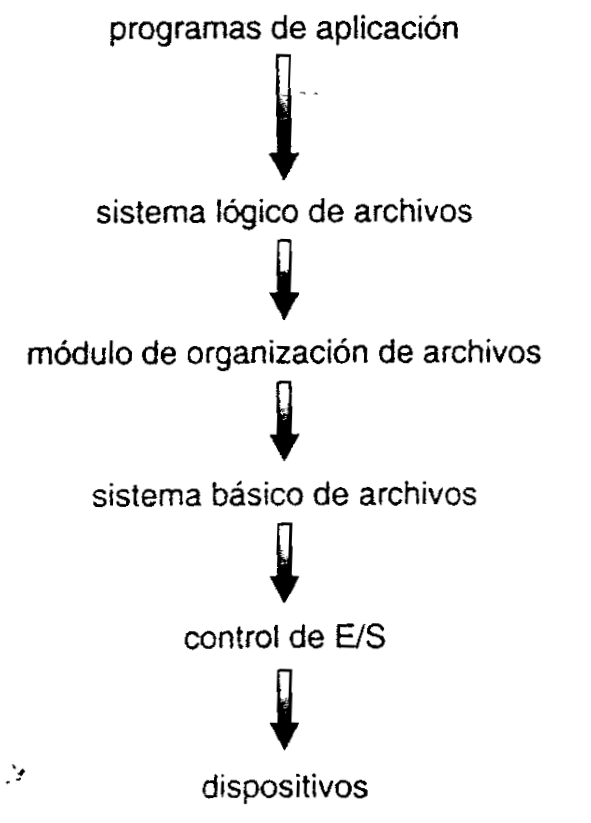
\includegraphics[height=0.36\textheight, keepaspectratio]{media/t04/capasSistemaArchivos.png}
    \caption{Arquitectura por capas de software de un subsistema de archivos \parencite[\S 11.1, p.\ 371]{silberschatz2006fundamentos}.}
    \label{fig:capasSistemaArchivos}
\end{figure}

\subsection{Capa de abstracción: el Sistema de Archivos Virtual (VFS)}
\label{subsec:capaAbstraccionVfs}

En un entorno computacional contemporáneo coexisten simultáneamente sistemas de archivos heterogéneos montados sobre una misma jerarquía de directorios: particiones raíz en ext4, volúmenes de respaldo en Btrfs, unidades externas en exFAT o NTFS, sistemas ópticos ISO 9660, recursos compartidos por red mediante NFS y pseudo-sistemas de archivos dinámicos del núcleo como \texttt{procfs} y \texttt{sysfs}. Para evitar que las aplicaciones deban programarse contra interfaces privativas de cada tecnología, el núcleo implementa una capa de indirección polimórfica denominada Sistema de Archivos Virtual (VFS, \textit{Virtual File System}) \parencite[\S 12.8, pp.\ 581--583]{stallings2018operating}.

El VFS define una interfaz orientada a objetos en C compuesta por cuatro estructuras canónicas fundamentales \parencite[\S 12.8, pp.\ 583--585]{stallings2018operating}:
\begin{itemize}[noitemsep, topsep=2pt]
    \item \textbf{Objeto de superbloque (\texttt{struct super\_block}):} Representa un sistema de archivos específico montado. Contiene metadatos del volumen (tamaño de bloque, banderas de solo lectura, identificador de dispositivo) y un puntero a su tabla de métodos polimórficos (\texttt{struct super\_operations}), permitiendo al núcleo invocar operaciones de montaje, desmontaje y asignación de inodos de forma agnóstica.
    \item \textbf{Objeto inodo (\texttt{struct inode}):} Representa la abstracción de un archivo o directorio individual en memoria. Alberga sus atributos persistentes y un vector de operaciones (\texttt{struct inode\_operations}) para manipular enlaces, permisos y nombres (\texttt{create}, \texttt{lookup}, \texttt{link}, \texttt{mkdir}).
    \item \textbf{Objeto entrada de directorio o \textit{dentry} (\texttt{struct dentry}):} Modela un nodo en la ruta jerárquica, asociando una cadena alfanumérica con su respectivo inodo. El VFS mantiene estas estructuras en una memoria caché de alta velocidad denominada \textit{dcache}, evitando exploraciones costosas en disco cada vez que un proceso resuelve rutas complejas como \texttt{/usr/bin/python3} \parencite[\S 12.8, p.\ 584]{stallings2018operating}.
    \item \textbf{Objeto archivo (\texttt{struct file}):} Representa una instancia de apertura dinámica en memoria asociada a un descriptor de proceso. Mantiene el puntero de desplazamiento actual (offset), las banderas de apertura (\texttt{flags}) y la tabla de operaciones de lectura, escritura y posicionamiento (\texttt{struct file\_operations}).
\end{itemize}

\subsection{Estructuras en disco y en memoria principal}
\label{subsec:estructurasDiscoMemoria}

La implementación física de un sistema de archivos requiere la coexistencia de estructuras permanentes almacenadas en el medio no volátil y estructuras volátiles en memoria RAM para la aceleración operativa \parencite[\S 11.2, pp.\ 372--374]{silberschatz2006fundamentos}:

\begin{itemize}[noitemsep, topsep=2pt]
    \item \textbf{Estructuras en almacenamiento secundario:}
    \begin{itemize}[noitemsep, topsep=1pt]
        \item \textit{Bloque de control de arranque (\textit{boot control block}):} Ocupa los primeros sectores del volumen o partición (p. ej., el sector de arranque de partición VBR o el registro maestro de arranque MBR). Contiene las instrucciones máquina ejecutadas por la interfaz de firmware para cargar el núcleo del sistema operativo.
        \item \textit{Bloque de control de volumen (\textit{volume control block}):} Denominado superbloque (\textit{superblock}) en UNIX/Linux o tabla maestra de archivos (MFT) en NTFS. Almacena la geometría del volumen, recuento de bloques totales y libres, tamaño del bloque de asignación y punteros a los mapas de espacio libre \parencite[\S 11.2, p.\ 373]{silberschatz2006fundamentos}.
        \item \textit{Estructura de directorios física:} Bloques reservados que enlazan los nombres simbólicos legibles por humanos con sus respectivos identificadores numéricos de inodo o punteros de bloque.
        \item \textit{Bloque de Control de Archivo (FCB):} Estructuras fijas (tabla de inodos en ext4) que albergan los atributos, marcas temporales y punteros a los bloques de datos de cada archivo \parencite[\S 8.5.1, p.\ 461]{carretero2001sistemas}.
    \end{itemize}
    \item \textbf{Estructuras dinámicas en memoria principal:}
    \begin{itemize}[noitemsep, topsep=1pt]
        \item \textit{Tabla de montaje del sistema:} Lista enlazada de todos los sistemas de archivos montados, enlazando puntos de montaje con sus superbloques activos.
        \item \textit{Caché de inodos y entradas de directorio (\textit{icache / dcache}):} Mantiene copias activas de los inodos recientemente consultados y de las ramas del árbol de directorios para evitar lecturas recurrentes de metadatos.
        \item \textit{Tabla global y tablas locales de archivos abiertos:} Coordinan los descriptores activos y punteros de desplazamiento entre procesos emparentados o independientes.
    \end{itemize}
\end{itemize}

\subsection{Métodos de asignación de bloques en almacenamiento secundario}
\label{subsec:metodosAsignacionBloques}

El módulo de organización de archivos debe resolver el problema crítico de cómo asignar bloques físicos de almacenamiento a los archivos lógicos en crecimiento. La eficiencia del acceso secuencial, la latencia del acceso aleatorio y el grado de fragmentación dependen del método adoptado \parencite[\S 11.4, pp.\ 380--388]{silberschatz2006fundamentos}:

\begin{enumerate}[noitemsep, topsep=2pt]
    \item \textbf{Asignación contigua (\textit{contiguous allocation}):} Cada archivo ocupa un conjunto de bloques consecutivos en el disco. Para acceder a cualquier bloque $n$ del archivo, basta sumar $n$ a la dirección del bloque inicial ($B_{dir} = B_{inicio} + n$), lo que otorga la máxima velocidad en acceso secuencial y directo, minimizando el desplazamiento de las cabezas lectoras en discos electromecánicos \parencite[\S 11.4.1, p.\ 380]{silberschatz2006fundamentos}. No obstante, genera fragmentación externa severa a medida que los archivos se borran y crean, requiriendo algoritmos de compactación periódicos. Asimismo, exige declarar o anticipar el tamaño final del archivo al momento de crearlo, produciendo fallos de asignación prematuros si el archivo supera el espacio continuo disponible \parencite[\S 12.7, p.\ 570]{stallings2018operating}.
    \item \textbf{Asignación enlazada (\textit{linked allocation}):} Cada archivo se representa como una lista enlazada de bloques físicos dispersos. Cada bloque almacena una porción de datos y un puntero físico hacia el siguiente bloque de la cadena; la entrada de directorio registra únicamente las direcciones del primer y último bloque \parencite[\S 11.4.2, p.\ 382]{silberschatz2006fundamentos}. Elimina por completo la fragmentación externa y permite que un archivo crezca indefinidamente mientras existan bloques libres en el volumen. Sin embargo, resulta ineficiente para el acceso directo: localizar el bloque $k$ requiere leer secuencialmente los $k-1$ bloques precedentes (complejidad $O(n)$). Además, presenta vulnerabilidad ante fallos de integridad: la pérdida o corrupción de un solo puntero provoca la pérdida irreparable del resto del archivo.
    \item \textbf{Asignación basada en tabla de asignación (FAT):} Variante optimizada de la asignación enlazada adoptada en MS-DOS y Windows. Los punteros de encadenamiento se extraen de los bloques de datos y se agrupan en una tabla contigua al inicio del disco denominada Tabla de Asignación de Archivos (FAT, \textit{File Allocation Table}) \parencite[\S 11.4.2, p.\ 384]{silberschatz2006fundamentos}. Al cargarse la tabla en memoria RAM, el acceso directo se acelera notablemente al recorrer la cadena de punteros en memoria principal sin incurrir en lecturas físicas a disco.
    \item \textbf{Asignación indexada (\textit{indexed allocation}):} Resuelve las deficiencias del acceso directo reuniendo todos los punteros a los bloques de datos de un archivo en una estructura dedicada denominada bloque de índice (\textit{index block}) \parencite[\S 11.4.3, p.\ 385]{silberschatz2006fundamentos}. El directorio almacena la dirección del bloque de índice, y el acceso a cualquier bloque lógico requiere una sola consulta directa a la tabla de índices, sin fragmentación externa. Para dar soporte a archivos de tamaños dispares, los sistemas implementan índices multinivel o esquemas combinados como el inodo tradicional de UNIX/Linux, el cual incorpora doce punteros directos, un puntero indirecto simple, un puntero indirecto doble y un puntero indirecto triple, posibilitando tanto el almacenamiento eficiente de archivos pequeños como el direccionamiento de archivos de escala multi-terabyte \parencite[\S 11.4.3, pp.\ 386--387]{silberschatz2006fundamentos}.
\end{enumerate}

La Tabla~\ref{tab:comparativaMetodosAsignacion} contrasta las propiedades operativas y estructurales de los métodos de asignación analizados.

\begin{table}[H]
\centering
\footnotesize
\renewcommand{\arraystretch}{1.0}
\renewcommand{\tabularxcolumn}[1]{m{#1}}
\setlength{\emergencystretch}{2em}
\caption{Comparativa técnica de métodos de asignación de espacio en almacenamiento secundario.}
\label{tab:comparativaMetodosAsignacion}
\begin{tabularx}{\textwidth}{>{\centering\arraybackslash}m{2.4cm} X X X}
\toprule
\textbf{Método} & \textbf{Eficiencia de acceso} & \textbf{Sobrecarga de almacenamiento} & \textbf{Fragilidad y fragmentación} \\
\midrule
\textbf{Contigua} & Óptima tanto en acceso secuencial como en aleatorio ($O(1)$). & Mínima: solo requiere dirección de inicio y longitud en el FCB. & Sufre fragmentación externa grave; requiere compactación periódica. \\
\addlinespace
\textbf{Enlazada pura} & Eficiente en acceso secuencial; muy deficiente en aleatorio ($O(n)$). & Pérdida de 4 u 8 bytes por bloque para alojar el puntero de enlace. & Nula fragmentación externa; muy vulnerable a corrupción de punteros. \\
\addlinespace
\textbf{Tabla FAT} & Rápida en secuencial; moderada en aleatorio mediante recorrido en RAM. & Tabla fija proporcional al número total de bloques del volumen. & Nula fragmentación externa; cuello de botella por concurrencia en la FAT. \\
\addlinespace
\textbf{Indexada (Inodo)} & Alta en secuencial y en aleatorio ($O(1)$ o $O(\log n)$ en multinivel). & Requiere bloques de índices dedicados incluso en archivos muy pequeños. & Nula fragmentación externa; gran tolerancia a fallos y alta escalabilidad. \\
\bottomrule
\end{tabularx}
\end{table}

\subsection{Gestión del espacio libre en disco}
\label{subsec:gestionEspacioLibre}

Para asignar bloques con rapidez cuando un archivo se crea o expande, el sistema operativo debe rastrear de forma continua cuáles bloques físicos están disponibles en el soporte persistente. Las tres técnicas elementales son \parencite[\S 11.5, pp.\ 388--391]{silberschatz2006fundamentos}:

\begin{itemize}[noitemsep, topsep=2pt]
    \item \textbf{Vector o mapa de bits (\textit{bit vector / bitmap}):} Cada bloque del disco se asocia a un bit individual (0 = libre, 1 = ocupado). Esta técnica es altamente compacta y permite que el núcleo localice el primer bloque libre o secuencias de bloques contiguos mediante instrucciones máquina especializadas de búsqueda de bits (\texttt{bsf} o \texttt{tzcnt} en arquitecturas x86\_64) \parencite[\S 11.5.1, p.\ 388]{silberschatz2006fundamentos}. Su eficiencia máxima exige mantener el mapa íntegramente en memoria RAM.
    \item \textbf{Lista enlazada de bloques libres:} Conecta todos los bloques disponibles entre sí mediante punteros almacenados en los propios bloques libres, requiriendo únicamente mantener en el superbloque un puntero al primer bloque libre \parencite[\S 11.5.2, p.\ 389]{silberschatz2006fundamentos}. No introduce sobrecarga de espacio adicional en disco, pero resulta lenta para asignaciones masivas contiguas.
    \item \textbf{Agrupación y recuento (\textit{grouping and counting}):} Almacena las direcciones de $n$ bloques libres en el primer bloque libre disponible, o registra pares estructurados formados por la dirección del primer bloque libre y el número de bloques continuos que le suceden (extents libres) \parencite[\S 11.5.3, p.\ 390]{silberschatz2006fundamentos}. Esta técnica es la base de los asignadores modernos en sistemas de archivos avanzados como ext4 y XFS, optimizando la asignación contigua a gran velocidad.
\end{itemize}

\section{Análisis comparativo de sistemas de archivos}
\label{sec:analisisComparativoSistemasArchivos}

\subsection{Criterios de evaluación y taxonomía arquitectónica}
\label{subsec:criteriosEvaluacionTaxonomia}

La evolución de los sistemas de archivos a lo largo de las últimas cuatro décadas refleja la constante adaptación del software de base frente al crecimiento exponencial en la capacidad de los medios persistentes, las demandas de concurrencia masiva en arquitecturas multiprocesador y la transición desde dispositivos electromecánicos hacia medios de estado sólido \parencite[\S 12.7, pp.\ 575--578]{stallings2018operating}. Para evaluar y clasificar técnicamente un sistema de archivos, el análisis de ingeniería examina cuatro dimensiones estructurales fundamentales:

\begin{enumerate}[noitemsep, topsep=2pt]
    \item \textbf{Representación de metadatos y direccionamiento:} Define cómo el sistema mapea la identidad lógica del archivo sobre los bloques físicos del medio. Los esquemas abarcan desde tablas de asignación globales lineales en memoria (FAT32, exFAT), tablas maestras de registros relacionales extensibles (MFT en NTFS), árboles combinados de nodos de índice con extensiones contiguas (inodos con extents en ext4 y XFS), hasta árboles B balanceados polimórficos (Btrfs, APFS) y estructuras unificadas de almacenamiento en depósitos virtuales (\textit{storage pools} en ZFS) \parencite[\S 11.4, pp.\ 384--387]{silberschatz2006fundamentos}.
    \item \textbf{Límites máximos de direccionamiento:} Determinados por el ancho de palabra binaria asignado a los punteros de bloque y campos de longitud en los descriptores del sistema. Las implementaciones transitan desde los 32 bits de FAT32 (limitado a archivos de 4 GiB), pasando por los 48 o 64 bits habituales en ext4, NTFS, XFS y APFS (capaces de direccionar magnitudes en el orden de los tebibytes y exbibytes), hasta alcanzar los 128 bits teóricos de ZFS, cuya capacidad de direccionamiento supera la masa atómica de los medios físicos concebibles \parencite{openzfs2024docs}.
    \item \textbf{Mecanismos de consistencia y tolerancia a fallos:} Establecen la capacidad del sistema para preservar la integridad ante interrupciones abruptas de energía o caídas del núcleo. La taxonomía divide los sistemas en tres grupos: aquellos sin bitácora que exigen revisiones completas fuera de línea mediante escaneos de disco (FAT32, exFAT); sistemas con bitácora (journaling) que registran previamente transacciones de metadatos o datos completos para una recuperación acelerada en el arranque (NTFS, ext4, XFS, HFS+) \parencite[\S 11.6, p.\ 392]{silberschatz2006fundamentos}; y sistemas modernos con paradigma de copia en escritura (CoW, Copy-on-Write) e integridad criptográfica de extremo a extremo, los cuales garantizan consistencia intrínseca y autorreparación de datos frente a degradación física silenciosa (bit rot) mediante sumas de comprobación (checksums) en árbol Merkle (ZFS, Btrfs, APFS) \parencite{openzfs2024docs}.
    \item \textbf{Capacidades avanzadas de gestión de almacenamiento:} Funcionalidades integradas en el propio sistema de archivos que eliminan la necesidad de capas intermedias de software, tales como compresión transparente en tiempo real (LZ4, ZSTD, LZNT1), cifrado criptográfico granular nativo por archivo o volumen (fscrypt, EFS, FileVault), creación de instantáneas (snapshots) de solo lectura o lectura/escritura en tiempo constante $O(1)$, clonación de archivos sin duplicación física de bloques y particionamiento en subvolúmenes flexibles \parencite{apple2020apfs, kernel2024btrfs}.
\end{enumerate}

\subsection{Tabla comparativa técnica de diez sistemas de archivos}
\label{subsec:tablaComparativaDiezSistemasArchivos}

La Tabla~\ref{tab:comparativaDiezSistemasArchivos} sintetiza los parámetros operativos, arquitecturas de metadatos, límites de direccionamiento, esquemas de consistencia y ámbitos de despliegue preferente de diez sistemas de archivos de amplia difusión en la industria computacional.

\begin{table}[!htbp]
\centering
\scriptsize
\renewcommand{\arraystretch}{1.1}
\renewcommand{\tabularxcolumn}[1]{m{#1}}
\setlength{\emergencystretch}{1.5em}
\caption{Análisis comparativo exhaustivo de diez sistemas de archivos contemporáneos.}
\label{tab:comparativaDiezSistemasArchivos}
\begin{tabularx}{\textwidth}{>{\centering\arraybackslash}m{1.3cm} >{\centering\arraybackslash}m{1.9cm} X X X X}
\toprule
\textbf{Sistema} & \textbf{Límites máx. (Archivo / Vol.)} & \textbf{Estructura de metadatos} & \textbf{Resiliencia y consistencia} & \textbf{Capacidades avanzadas} & \textbf{Ámbito de despliegue principal} \\
\midrule
\textbf{FAT32} & 4 GiB / \newline 2 TiB & Tabla de asignación de archivos de 32 bits (FAT); directorio plano de 32 bytes con soporte VFAT. & Sin bitácora; susceptible a inconsistencias tras apagones; requiere escaneo con FSCK o CHKDSK. & Compatibilidad universal multiplataforma; sin soporte de permisos nativos ni cuotas de usuario. & Memorias USB heredadas, tarjetas SD, partición de arranque UEFI (ESP). \\
\addlinespace
\textbf{exFAT} & 16 EiB / \newline 128 PiB & Tabla FAT simplificada con mapa de bits de asignación contigua para optimizar archivos sin fragmentar. & Sin bitácora; soporte transaccional opcional en TexFAT; menor fragilidad que FAT32. & Nombres de archivo Unicode hasta 255 caracteres; sin compresión ni permisos POSIX nativos. & Tarjetas de memoria SDXC de alta capacidad y unidades externas de intercambio. \\
\addlinespace
\textbf{NTFS} & 16 TiB / \newline 256 TiB & Tabla Maestra de Archivos (MFT) como base relacional; descriptores de archivo en registros de 1 KiB. & Bitácora transaccional para metadatos mediante \texttt{\$LogFile}; recuperación atómica en fases. & Listas de control de acceso (ACL), flujos alternos (ADS), cifrado EFS, compresión y cuotas. & Partición de sistema y almacenamiento interno en Microsoft Windows NT/10/11. \\
\addlinespace
\textbf{ext4} & 16 TiB / \newline 1 EiB & Inodos de 256 bytes por grupos de bloques; direccionamiento con árboles balanceados de extents. & Bitácora JBD2 con tres niveles (journal, ordered, writeback); checksums en metadatos. & Asignación diferida, preasignación contigua \texttt{fallocate()}, cifrado nativo fscrypt. & Sistema predeterminado en la mayoría de distribuciones GNU/Linux de escritorio y servidor. \\
\addlinespace
\textbf{Btrfs} & 16 EiB / \newline 16 EiB & Estructura multirrámica basada en árboles B+ genéricos bajo copia en escritura (CoW). & Integridad de extremo a extremo con sumas CRC32C/SHA256 en datos y metadatos; autorreparación. & Instantáneas gravables $O(1)$, subvolúmenes dinámicos, compresión transparente zstd/LZO. & Partición raíz en Fedora y openSUSE; servidores NAS e infraestructuras contra corrupción. \\
\addlinespace
\textbf{XFS} & 8 EiB / \newline 8 EiB & Grupos de asignación (AG) paralelos e independientes; inodos dinámicos y árboles B+ de extents. & Bitácora circular de metadatos de alto rendimiento; recuperación inmediata; checksums v5. & Escalabilidad extrema para E/S paralela masiva, asignación diferida y cuotas por proyecto. & Almacenamiento estándar en Red Hat Enterprise Linux (RHEL) y servidores de bases de datos. \\
\addlinespace
\textbf{ZFS} & 16 EiB / \newline 256 ZiB & Fusión de sistema de archivos y administrador de volúmenes (zpools); árbol Merkle de 128 bits. & CoW transaccional estricto; suma de comprobación criptográfica por bloque; repara bit rot. & Instantáneas y clones instantáneos, compresión dinámica LZ4/ZSTD, desduplicación, RAID-Z. & Almacenamiento corporativo de misión crítica, servidores TrueNAS, FreeBSD e Illumos. \\
\addlinespace
\textbf{HFS+} & 8 EiB / \newline 8 EiB & Archivo de catálogo jerárquico basado en árbol B*; bifurcaciones de recursos y datos separadas. & Bitácora de metadatos en diario; previene el escaneo exhaustivo del catálogo en arranque. & Codificación Unicode UTF-8 descompuesta, compresión nativa HFS, listas de control de acceso. & Sistema predeterminado en entornos Apple históricos (Mac OS 8.1 hasta macOS Sierra 10.12). \\
\addlinespace
\textbf{APFS} & 8 EiB / \newline 8 EiB & Árboles B+ adaptados a memorias flash SSD; espacio compartido dinámico en un único contenedor. & Redirección en escritura para atomicidad transaccional sin bitácora; sumas en metadatos. & Clonación de archivos sin duplicación, instantáneas atómicas, cifrado nativo multi-clave. & Sistema nativo y obligatorio en todos los dispositivos Apple contemporáneos (macOS, iOS). \\
\addlinespace
\textbf{F2FS} & 3.93 TiB / \newline 16 TiB & Estructura en registros segmentados (\textit{Log-Structured File System}) optimizada para flash NAND. & Puntos de control periódicos (checkpointing) y registros de reversión (\textit{roll-forward}). & Separación de datos calientes/fríos, recolección de basura adaptativa, soporte TRIM y compresión. & Teléfonos inteligentes Android, dispositivos embebidos y unidades de estado sólido de consumo. \\
\bottomrule
\end{tabularx}
\end{table}

\subsection{Análisis de paradigmas de consistencia y almacenamiento}
\label{subsec:analisisParadigmasConsistencia}

El diseño interno de un sistema de archivos define la estrategia adoptada para conciliar el rendimiento en operaciones de entrada/salida con la preservación incondicional de la coherencia de los datos ante fallos imprevistos de hardware o interrupciones de energía \parencite[\S 11.6, pp.\ 392--394]{silberschatz2006fundamentos}. En la práctica de la ingeniería computacional destacan tres grandes paradigmas:

\begin{enumerate}[noitemsep, topsep=2pt]
    \item \textbf{Paradigma de bitácora transaccional (journaling):} En los sistemas convencionales con actualización en el sitio (update-in-place) como ext4 o NTFS, modificar un archivo exige realizar múltiples escrituras independientes en sectores dispersos del disco (bloques de datos, mapas de bits, inodos y directorios). Si el suministro eléctrico se interrumpe antes de completar la secuencia, el volumen queda inconsistente y requiere escaneos prolongados con \texttt{fsck} o \texttt{chkdsk} \parencite[\S 12.9, pp.\ 586--588]{stallings2018operating}. El journaling resuelve este problema reservando un área circular en disco denominada bitácora (journal). Antes de persistir cambios en las estructuras finales, el núcleo agrupa las operaciones en una transacción atómica y la registra de manera secuencial en la bitácora. Tras confirmarse la escritura física de la transacción (\textit{commit}), el núcleo transfiere de forma asíncrona las modificaciones a sus ubicaciones finales en disco (checkpointing). En caso de caída, durante el arranque el núcleo examina únicamente la bitácora: descarta transacciones incompletas y reaplica las transacciones confirmadas pendientes en segundos (\textit{replay}), garantizando consistencia inmediata \parencite[\S 11.6, p.\ 393]{silberschatz2006fundamentos}.
    \item \textbf{Paradigma de copia en escritura (Copy-on-Write, CoW) y árboles Merkle:} Sistemas modernos como ZFS, Btrfs y APFS descartan la actualización en el sitio. Bajo CoW, los bloques de datos y metadatos existentes jamás se sobreescriben. Cuando un proceso modifica información, el asignador reserva un nuevo bloque físico libre donde graba la versión actualizada. La referencia en el nodo padre del árbol se actualiza en cascada de forma ascendente hasta alcanzar la raíz del árbol (\textit{uberblock} o superbloque de anclaje) \parencite{openzfs2024docs}. La confirmación de la transacción se reduce a una sola escritura atómica del puntero de raíz. Si ocurre una interrupción eléctrica, la raíz anterior sigue referenciando la versión coherente previa, prescindiendo de bitácoras de recuperación. Este esquema hace posible generar instantáneas (snapshots) atómicas en tiempo $O(1)$ congelando la raíz temporal. Con sumas de comprobación criptográficas incrustadas en los punteros padres de cada bloque, el sistema detecta y autorrepara la corrupción silenciosa de datos (bit rot) sobre arreglos redundantes \parencite{openzfs2024docs, kernel2024btrfs}.
    \item \textbf{Paradigma estructurado en registros (\textit{Log-Structured}) para memorias flash:} Las unidades de estado sólido basadas en tecnología flash NAND operan bajo restricciones físicas: leen y programan en páginas (de 4 a 16 KiB), pero borran únicamente en bloques de borrado completos (\textit{erase blocks}, de 2 a 8 MiB) \parencite{lee2015f2fs}. La sobreescritura aleatoria tradicional fuerza al controlador a ejecutar ciclos de lectura-borrado-reescritura, disparando el factor de amplificación de escritura (WAF, \textit{Write Amplification Factor}) y reduciendo la vida útil del silicio. Sistemas como F2FS transforman todas las escrituras aleatorias en un flujo estrictamente secuencial de datos en segmentos limpios, separando la información en flujos calientes, tibios y fríos. Mediante recolección de basura adaptativa en segundo plano y órdenes TRIM de SATA/NVMe, F2FS minimiza la degradación y optimiza el rendimiento sostenido del medio \parencite{lee2015f2fs}.
\end{enumerate}

\section{Sistemas de archivos en sistemas operativos contemporáneos}
\label{sec:sistemasArchivosContemporaneos}

La selección del sistema de archivos en los sistemas operativos responde a criterios de compatibilidad, tolerancia a fallos, seguridad del núcleo y optimización para medios persistentes. A continuación se examina la arquitectura de almacenamiento en cuatro plataformas contemporáneas.

\subsection{GNU/Linux Mint 21.2 «Victoria»}
\label{subsec:linuxMintVictoria}

GNU/Linux Mint 21.2 («Victoria»), basado en Ubuntu 22.04.2 LTS con núcleo Linux 5.15 LTS, adopta \textbf{ext4} (\textit{Fourth Extended Filesystem}) como sistema predeterminado en la raíz (\texttt{/}) \parencite{linuxmint2023victoria}. Emplea inodos de 256 bytes, árboles de extensiones (extents) y bitácora JBD2 en modo \texttt{data=ordered}, garantizando que los datos alcancen el medio persistente antes de asentar metadatos \parencite{kernel2024ext4}. El intercambio opera mediante archivo dinámico (\texttt{/swapfile}) sobre ext4 vía \texttt{fibmap}, con el arranque UEFI en \textbf{FAT32} sobre la partición ESP (\texttt{/boot/efi}).

Mint 21.2 integra la herramienta de restauración \textbf{Timeshift} \parencite{linuxmint2023victoria}. Con ext4 opera en modo RSYNC mediante enlaces duros (\textit{hard links}) para capturar instantáneas diferenciales sin duplicar archivos intactos. Alternativamente, soporta \textbf{Btrfs} con subvolúmenes \texttt{@} (raíz) y \texttt{@home} (usuarios); bajo este esquema, Timeshift conmuta al modo nativo BTRFS para capturar instantáneas CoW en tiempo constante $O(1)$, posibilitando la reversión inmediata del sistema desde GRUB ante actualizaciones fallidas \parencite{linuxmint2023victoria}.

\subsection{Ubuntu 23.04 «Lunar Lobster»}
\label{subsec:ubuntuLunarLobster}

Ubuntu 23.04 («Lunar Lobster»), con núcleo Linux 6.2 e instalador Subiquity/Flutter, mantiene \textbf{ext4} como sistema primario en escritorio y servidores \parencite{canonical2023ubuntu}. Opera con direccionamiento de 64 bits (\texttt{64bit}), asignación diferida (\textit{delayed allocation}) y sumas CRC32C (\texttt{metadata\_csum}), blindando inodos y mapas de bloques frente a corrupción silenciosa \parencite{kernel2024ext4}. Conserva soporte para \textbf{OpenZFS} (\textit{ZFS on root}) con depósitos (zpools) \texttt{rpool} y \texttt{bpool}, permitiendo a \texttt{zsys} capturar instantáneas previas a cada invocación de \texttt{apt} \parencite{canonical2023ubuntu, openzfs2024docs}.

En Ubuntu 23.04, el sistema comprimido de solo lectura \textbf{Squashfs} distribuye aplicaciones en paquetes \textbf{Snap} vía \texttt{snapd} \parencite{canonical2023ubuntu, kernel2024squashfs}. Aplicaciones como Firefox no residen dispersas en \texttt{/usr}, sino en imágenes Squashfs inmutables (comprimidas con XZ o LZO) asociadas en el arranque a dispositivos de bucle invertido (\texttt{/dev/loop}) y montadas bajo \texttt{/snap/}\allowbreak\texttt{paquete/}\allowbreak\texttt{revisión}. Este confinamiento con AppArmor y espacios de nombres (\textit{namespaces}) asegura aislamiento estricto, con el arranque UEFI en \textbf{FAT32} sobre ESP \parencite{canonical2023ubuntu}.

\subsection{Apple macOS 10.15 «Catalina»}
\label{subsec:macosCatalina}

macOS 10.15 («Catalina») adoptó \textbf{APFS} (\textit{Apple File System}) sustituyendo a HFS+ en el almacenamiento interno \parencite{apple2020apfs}. Catalina redefinió la arquitectura mediante \textbf{volúmenes gemelos dedicados} en un contenedor compartido APFS (\textit{shared container}): el volumen de sistema (\texttt{Macintosh HD}), montado de solo lectura en la raíz \texttt{/} bajo protección SIP (\textit{System Integrity Protection}) con el núcleo XNU y marcos esenciales (\texttt{/System}); y el volumen de datos (\texttt{Macintosh HD - Data}), montado en \texttt{/System/}\allowbreak\texttt{Volumes/}\allowbreak\texttt{Data} para usuarios (\texttt{/Users}), aplicaciones (\texttt{/Applications}) y configuraciones (\texttt{/private}) \parencite{apple2020apfs}.

Para asegurar compatibilidad con POSIX y un espacio de nombres continuo, Apple implementó \textbf{enlaces firmes sintéticos (\textit{firmlinks})} \parencite{apple2020apfs}. Un \textit{firmlink} es un túnel bidireccional en el núcleo y metadatos de APFS que enlaza de forma transparente directorios de solo lectura con sus pares en datos (proyectando \texttt{/Users} hacia \texttt{/System/}\allowbreak\texttt{Volumes/}\allowbreak\texttt{Data/}\allowbreak\texttt{Users}). La seguridad física del contenedor se complementa con \textbf{FileVault 2}, mediante claves AES-XTS independientes gestionadas por el coprocesador Apple T2 \parencite{apple2020apfs}.

\subsection{Microsoft Windows 10}
\label{subsec:microsoftWindows10}

En Windows 10 (22H2), el sistema de archivos obligatorio para el sistema (\texttt{C:}) es \textbf{NTFS} (\textit{New Technology File System}, versión 3.1), exigido por \texttt{winload.efi} con clústeres de 4 KiB \parencite{microsoft2024ntfs}. NTFS articula la Tabla Maestra de Archivos (MFT, Master File Table) en registros de 1024 bytes (con atributos residentes en archivos pequeños), la bitácora \texttt{\$LogFile} y el registro USN Journal (\texttt{\$UsnJrnl}) para atomicidad transaccional, y el control de acceso por listas DACL/SACL con identificadores SID, cifrado nativo EFS y cifrado completo mediante \textbf{BitLocker} \parencite{microsoft2024ntfs, stallings2018operating}.

Para volúmenes secundarios, Windows 10 emplea una partición ESP en \textbf{FAT32} para UEFI, soporta \textbf{exFAT} en medios extraíbles e incorpora \textbf{ReFS} (\textit{Resilient File System}) en Workstation y Enterprise para depósitos masivos (\textit{Storage Spaces}) con CoW e integridad verificable, sin arranque ni compresión nativa \parencite{microsoft2024refs}. La Tabla~\ref{tab:sistemasArchivosSistemasOperativos} resume los roles y subsistemas analizados.

\begin{table}[H]
\centering
\scriptsize
\captionsetup{skip=4pt}
\renewcommand{\arraystretch}{0.85}
\renewcommand{\tabularxcolumn}[1]{m{#1}}
\setlength{\tabcolsep}{3pt}
\setlength{\emergencystretch}{1.5em}
\caption{Sistemas de archivos implementados en sistemas operativos contemporáneos.}
\label{tab:sistemasArchivosSistemasOperativos}
\begin{tabularx}{\textwidth}{>{\centering\arraybackslash}m{2.3cm} >{\centering\arraybackslash}m{2.4cm} >{\centering\arraybackslash}m{2.4cm} X}
\toprule
\textbf{Sistema Operativo} & \textbf{Partición raíz} & \textbf{Partición datos} & \textbf{Tecnologías y subsistemas secundarios} \\
\midrule
\textbf{GNU/Linux Mint 21.2} & ext4 (predet.) / Btrfs & ext4 / Btrfs (\texttt{@home}) & Instantáneas Timeshift (RSYNC o CoW), \texttt{swapfile} en ext4, FAT32 en ESP. \\
\textbf{Ubuntu 23.04} & ext4 (predet.) / OpenZFS & ext4 / OpenZFS & Paquetes Snap sobre Squashfs inmutable (\texttt{/dev/loop}), \texttt{zsys}, FAT32 en ESP. \\
\textbf{macOS 10.15 Catalina} & APFS (\textit{read-only}) & APFS (\texttt{Data}) & Túneles sintéticos firmlinks, cifrado FileVault 2 (Apple T2), SIP. \\
\textbf{Microsoft Windows 10} & NTFS obligatorio (v3.1) & NTFS & Bitácora \texttt{\$LogFile}, registro USN, BitLocker, ReFS en Workstation, FAT32 en ESP. \\
\bottomrule
\end{tabularx}
\end{table}

\section{Conclusiones personales}
\label{sec:conclusionesPersonales}

La investigación y el análisis estructural confirman que el sistema de archivos no constituye un organizador pasivo de datos, sino uno de los subsistemas de abstracción más complejos y críticos del sistema operativo. La transición desde registros rígidos hacia el flujo continuo no estructurado de bytes (stream of bytes), consolidado por UNIX y POSIX, redefinió la relación entre el núcleo y el espacio de usuario. Al delegar la interpretación en las aplicaciones y reservar al núcleo la asignación eficiente, protección de memoria y multiplexación de descriptores, se unificó el tratamiento de archivos ordinarios, tuberías y controladores. Asimismo, el Sistema de Archivos Virtual (VFS) demostró que el desacoplamiento polimórfico entre llamadas al sistema estandarizadas y estructuras físicas en disco es indispensable para garantizar la interoperabilidad en entornos heterogéneos con múltiples tecnologías coexistiendo en un mismo espacio jerárquico.

El análisis de paradigmas de consistencia confirma una transformación sustancial en el almacenamiento persistente. Frente a la actualización en el sitio (update-in-place) y la sobrecarga por doble escritura del journaling tradicional (\texttt{fsck} o \texttt{chkdsk}), las arquitecturas basadas en copia en escritura (CoW, Copy-on-Write) y árboles balanceados Merkle —materializadas en ZFS, Btrfs y APFS— establecen un estándar superior de resiliencia. Al registrar cada modificación como una nueva asignación física atómica propagada hacia la raíz del volumen, erradican los estados corruptos intermedios. Esta propiedad garantiza consistencia inmediata ante caídas abruptas y optimiza el respaldo al permitir instantáneas (snapshots) y clonación en tiempo constante $O(1)$ sin duplicar bloques.

La evolución del software de base permanece ligada a la física del hardware. La sustitución de discos rotatorios por memorias flash NAND derribó premisas algorítmicas de mitigación de retardos mecánicos. Las memorias de estado sólido imponen restricciones: la asimetría entre páginas de programación y bloques de borrado exige algoritmos que minimicen el factor de amplificación de escritura. Tecnologías como F2FS demuestran que el sistema de archivos debe dialogar con la capa FTL, sincronizando la recolección de basura y las órdenes TRIM para extender la durabilidad del silicio. Paralelamente, los sistemas operativos contemporáneos integran la seguridad e inmutabilidad en el núcleo: volúmenes gemelos con firmlinks en macOS Catalina, imágenes Squashfs inmutables en Snap bajo Ubuntu, y bitácoras con USN Journal en Windows 10. En conclusión, el sistema de archivos trasciende la intermediación de bloques para afianzarse como una plataforma integral de integridad, cifrado y resiliencia determinista.

\nocite{*}
\newpage
\setlength\bibitemsep{0.30em}
\printbibliography[heading=bibintoc, title={Referencias}]

\end{document}
